\documentclass[letterpaper,11pt,twocolumn]{article}
\usepackage{graphicx,common}
\usepackage[nonamebreak,numbers,sort&compress]{natbib}
\bibliographystyle{plainnat}
\setlength{\textwidth}{6.5in} 
\setlength{\textheight}{9in}
\setlength{\topmargin}{-0.0625in} 
\setlength{\oddsidemargin}{0in}
\setlength{\evensidemargin}{0in} 
\setlength{\headheight}{0in}
\setlength{\headsep}{0in} 
\setlength{\hoffset}{0in}
\setlength{\voffset}{0in}
\makeatletter
\renewcommand{\section}{\@startsection%
{section}{1}{0mm}{-\baselineskip}%
{0.5\baselineskip}{\normalfont\Large\bfseries}}%
\makeatother
\newcommand{\apj}{ApJ}
\newcommand{\apjs}{ApJS}
\newcommand{\apjl}{ApJL}
\newcommand{\aap}{A{\&}A}
\newcommand{\aaps}{A{\&}AS}
\newcommand{\apss}{Ap{\&}SS}
\newcommand{\mnras}{MNRAS}
\newcommand{\aj}{AJ}
\newcommand{\araa}{ARAA}
\newcommand{\pasp}{PASP}
\begin{document}
\pagestyle{plain}
\pagenumbering{arabic}
\begin{center}
\bfseries\uppercase{The Hyperluminous Infrared Galaxy IRAS 09104+4109: An Extreme Brightest Cluster Galaxy}
\end{center}
\section{Introduction}
In half of all clusters of galaxies, the gas in their cores has a
radiative cooling time $<$ H$_{0}^{-1}$. Thus, one expects layers
of cooling, dense, low pressure gas to collapse under the
high pressure, hot gas at larger radii initiating a flow of cool
gas into the core
(\cite{1977MNRAS.180..479F},\cite{1977ApJ...215..723C}). In the
cooling flow scenario, one also expects to find a continuum of
gas temperatures in cluster cores down to fractions of an eV
\cite{1994MNRAS.266..399F}. However, observations do not find
gas at less than $\sim 1/3$ of the ambient cluster temperature and
direct evidence, such as gas condensing out of the ICM, for the hypothesized cooling
flows has never been found thus creating a ``cooling flow problem''
\cite{1995ApJ...452..164V}.
Some mechanism must be acting within cluster cores to retard a
continuous cooling gas phase.

The ``cooling flow problem" has a viable 
solution in the form of AGN feedback
(\cite{1995MNRAS.276..663B},\cite{2005ApJ...634..955V}), but
the details of AGN feedback cycles and instigation are still
unresolved \cite{2002MNRAS.330..329B}. Most models of AGN
feedback rely on quenched cooling from heat supplied by kinetic
energy generated from a central supermassive black hole (cSMBH) of the brightest cluster
galaxy (BCG). Gas is dumped onto the cSMBH, which initiates an AGN
feedback cycle, and is followed by ejection of high energy particles which create
cavities in the X-ray gas (``bubbles''). The work done by these bubbles on
the surrounding ICM, $W_{bubble} = pV$, goes into displacing ICM gas around and
into the bubble wake where the
gravitational potential energy is then released as enthalpy \cite{2004ApJ...607..800B}.
Heating of the ICM increases the entropy of the gas, but not necessarily
its equilibrium temperature, which is primarily determined by depth of the gravitational potential. This
overall heating and cooling cycle is imprinted on the cluster gas
entropy, here defined to be $K \equiv kTn_{elec}^{-2/3}$, where T is the gas temperature
and n$_{elec}$ is the electron density (\cite{2002ApJ...576..601V},
\cite{2005RvMP...77..207V}). The quantities T and n$_{elec}$ can be
measured from X-ray data thereby giving a direct measure of the
cluster thermal history via entropy.

\begin{figure}[t]
\begin{minipage}[t]{0.9\linewidth}
\centering
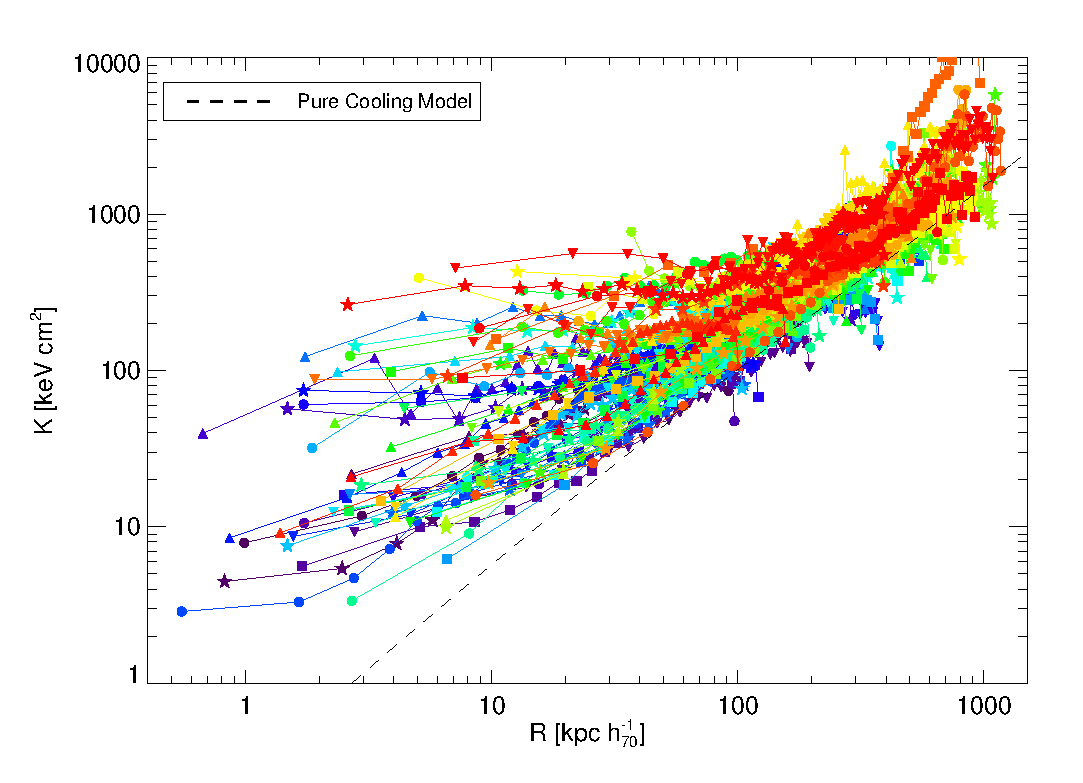
\includegraphics[width=\textwidth, trim=28mm 10mm 30mm 17mm, clip]{splots}
\caption{
Plotted are the radial entropy profiles for 68 of the
200+ clusters in the PhD sample of Cavagnolo 2008 (in prep.). The
curves are color coded purple=coolest to red=hottest. The coolest cluster in
the sample is MKW4 at kT=2.06 keV and the hottest cluster is Abell
2163 at kT=12.1 keV.
}
\label{fig:ent}
\end{minipage}
\end{figure}

Figure \ref{fig:ent} shows the
radial entropy profiles for a portion of the clusters analyzed in the PhD
thesis work of Cavagnolo 2008 (in preparation), which is
utilizing 200+ {\textit{Chandra}} archival observations of clusters of
galaxies to study their entropy profiles and distributions. The
profiles show a marked resemblance irrespective of global cluster
temperatures ranging from 2-12 keV. In this work, we have found a
strong correlation of increasing central entropy with decreasing radio
luminosity, indicating the AGN duty cycle is tied to the ICM entropy
distribution.

\section{IRAS 09104+4109: An Extreme BCG}
At z $< 0.5$ and $L > 10^{11} L_{\odot}$ the most common extragalactic
objects are infrared galaxies. Among this population are a subset
of ultraluminous infrared galaxies (ULIRGs) with $L_{IR} \geq 10^{12} L_{\odot}$,
and an even more rare subset of hyperluminous infrared galaxies
(HLIRGs) with $L_{IR} \geq 10^{13} L_{\odot}$. IRAS 09104+4109
classifies as a HLIRG with a $L_{IR} \approx 10^{13} L_{\odot}$. Most all ULIRGs and
HLIRGs are interacting/merging spirals or relics of recent
mergers. Unlike fellow HLIRGs, IRAS 09104+4109 is the BCG in
the flattened, Abell richness class 2 cluster MACS J0913.7+4056. Even more
peculiar is that unlike most all BCGs found in rich clusters, 99\% of
IRAS 09104+4109's bolometric luminosity comes longward of 1$\mu$m and peaks between
5-60$\mu$m \cite{1988ApJ...328..161K}. This enormous IR luminosity is
attributed to an obscured Seyfert type 2 AGN with a large dust torus
lying between the broad-line and narrow-line regions
(\cite{1993ApJ...415...82H}, \cite{1999ApJ...512..145H}) and not to
starbursts, as is the case for many luminous infrared galaxies.
The fuel sources for the central AGN may be the optical nebular 
filaments and companion galaxies within 30kpc
of the BCG which are being stripped of their gas and cannibalized
\cite{1999Ap&SS.266..113A}. The presence of dust
within these filaments and substructures may rule out the hot intracluster
medium as their origin (\cite{2000AJ....120..562T},\cite{1993ApJ...414L..17D}) because
of the short sputtering time for dust in hot gas \cite{1979ApJ...231...77D}. Of all
objects in the IRAS catalog, 09104+4109 hosts the most powerful radio
source, a borderline FRII/FRI with $P_{1.4GHz} = 3.2\times10^{24}$ W
Hz$^{-1}$. Yet because of the steep radio spectrum and huge IR luminosity, 
the radio source would be classified as ``quiet''
at higher frequencies. \cite{1999ApJ...512..145H} conclude
the radio source has undergone a recent ($< 70$ kyr) merger event or cataclysmic
occurrence which has altered the beaming direction of the central
AGN. As a result, the radio lobes are no longer receiving
power from the AGN and a new jet axis has been established. In
addition, only three other objects in the IRAS catalog are comparable
to 09104+4109 in luminosity and
they all lie at redshifts which would require very long exposure
observations to attain spectroscopic quality signal to noise: IRAS
15307+3252 (z=0.93), IRAS 16347+703 (z=1.334),
and IRAS 10214+4724 (z=2.29).

\begin{figure}
%\begin{center}
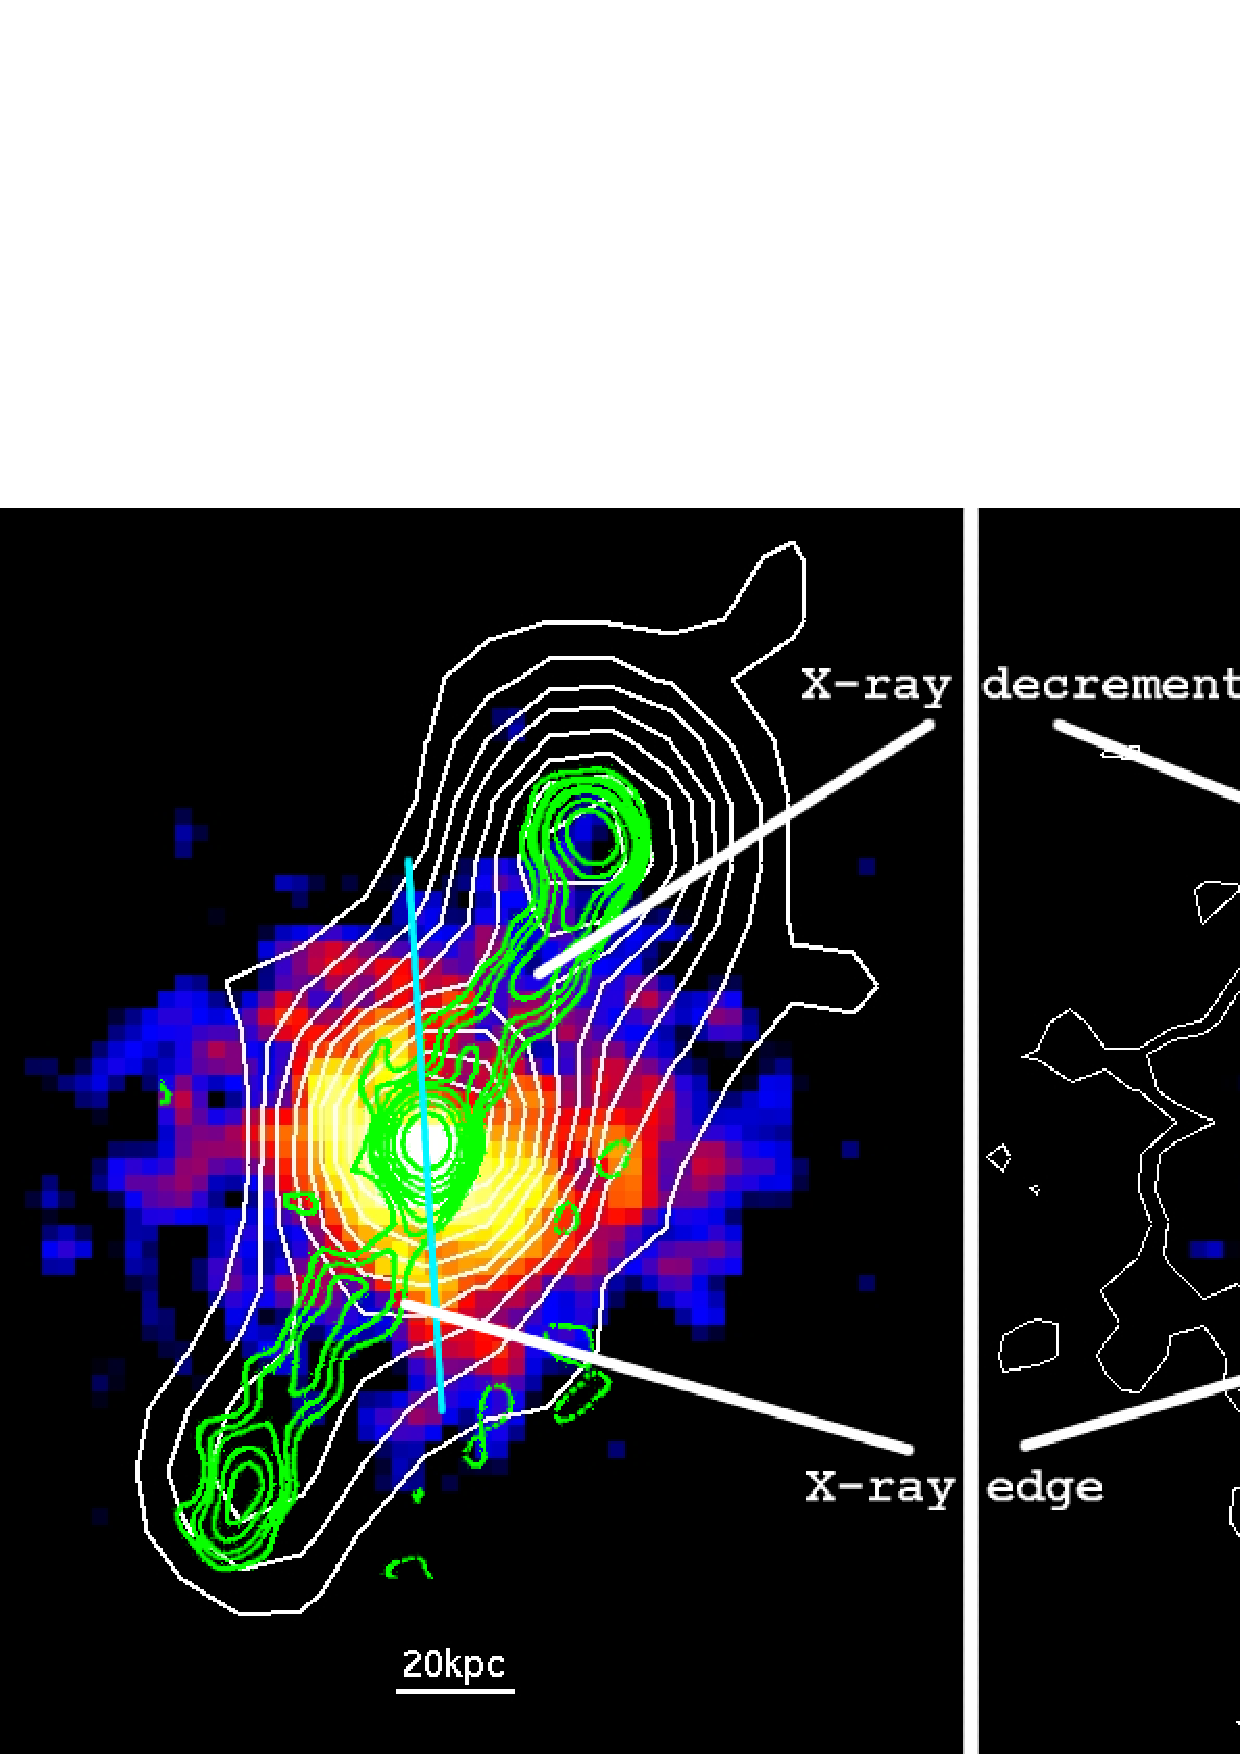
\includegraphics[scale=0.22]{chan_vla_utrao}
\caption{The left panel shows the
existing {\textit{Chandra}} data with low resolution
20 cm VLA First contours (white), high resolution 20 cm VLA contours
from \cite{1993ApJ...415...82H} (green), and the new AGN outflow axis as
determined from the bipolar ionization cone discussed in 
\cite{1999ApJ...512..145H} (light blue line). The right panel shows the same
{\textit{Chandra}} image with X-ray contours and 
green elliptical regions highlighting X-ray surface brightness decrement and X-ray
surface brightness edge.}
%\end{center}
\label{fig:chanrad}
\end{figure}
\subsection{Bubbles in IRAS 09104+4109}
We were surprised to find a probable X-ray
cavity $\approx 30$ kpc NW of the BCG in a cluster
at z$ > 0.4$. The highest redshift bubble published to date is in
RBS 797 at z=0.350 \cite{2001A&A...376L..27S}. The X-ray decrement
was mentioned in passing by the PIs of the first {\textit{Chandra}}
observation, \S{3.1} in \cite{2001MNRAS.321L..15I}. Analysis of the
publicly-available, low-resolution
radio data from VLA First reveals a suggestive alignment of the NW radio
jet and the observed X-ray decrement (Fig. \ref{fig:chanrad}). X-ray
emission in the opposite direction and on the opposing side of the nuclear
region is also suspiciously flat and coincident with the other pole of
the radio jet. We suggest the NW decrement is the
stem of a larger bubble and the SE plateau results from interaction of
the ICM with another large bubble. The
detection of dust
in the environment surrounding these two features
indicates shocking is not playing a major role in heating of the
gas. This supports the case for bubbles rather than chance superposition of
shocked regions because the rims of bubbles
are dense and cold, not dense and hot as would be the case with shocks.
Coincidence of the radio jets and two prominent X-ray features is
an unlikely chance projection of overdense regions which have no
underlying physical connection.
If confirmed, these would be the highest redshift bubbles found to
date. Bubbles are a way of indirectly studying
heating of the ICM by AGN, and in the case of IRAS 09104+4109 we
have the chance to see how a rare and peculiar object fits into the
now widely used model of quenching cooling in clusters by AGN feedback.

\subsection{Scientific Questions}
Calling the 100 kpc around IRAS 09104+4109 lively is an
understatement. The flurry of activity surrounding the AGN combined
with a peculiar amalgam of physical properties makes IRAS 09104+4109 a
rare, interesting, and extreme object. One can ask many questions about the
large scale structure of this object. In Figure \ref{fig:ent},
clusters with the lowest central
entropy have the most luminous radio sources; the radio source in IRAS
09104+4109 is undergoing a transition from powerful FRII to being mostly radio-quiet/FRI and
thus we would expect the radial entropy distribution slope to be relatively flat and
bare a resemblance to other radio-quiet clusters,
e.g. \cite{2005ApJ...630L..13D}. But, this object is no where near as
relaxed as other radio-quiet clusters and based on the X-ray
morphology we would expect the entropy profile to be steeper,
resembling other ``dynamic'' clusters, such as 2A0335+096 or Abell
2029 \cite{2006ApJ...643..730D}. So we ask:\\
1) To which regime does the cluster housing IRAS 01904+4109 more closely belong,
radio-quiet or dynamically active? Can we definitively classify this
object as being in a short lived and elusive transitional phase of
galaxy, cluster, and AGN evolution?\\
2) Has the change in beaming direction of the radio source created
multiple bubbles?\\
3) What can the energetic properties of these bubbles
tell us about the connection between the present phase of AGN feedback
and epochs of feedback which may have occurred long prior and have now
deposited their energy at large radii thus changing the entropy
structure there?\\
4) Knowing of a recent change in the dynamics of the radio source, can we
detect this change by comparing the 2-dimensional entropy and pressure structure at
r $< 70$ kpc of the AGN and r $> 70$ kpc?\\
-- The duty cycle of AGNs is believed to be $\sim$ 10$^8$ yr, do we
find signatures of previous feedback cycles at large radii to
constrain the feedback timescale and compare it with other clusters?\\
Answers to these questions require resolving the extended X-ray
emission at radii greater than 70 kpc which we cannot do with the
existing {\textit{Chandra}} observation.

\section{Proposed Research}
\subsection{Why not use existing data?}
Using CIAO 3.4.1.1 and CALDB 3.3.0.1, we analyzed the existing ACIS-S3
observation taken 1999-11-03 by Fabian, which was originally used to
examine reflected X-ray emission of the AGN \cite{2001MNRAS.321L..15I}.
The nominal 9.1 ks exposure shows contamination by two strong flares which reduce
the usable exposure time to $\approx$5 ks. However, there is
an additional long duration, soft flare which is not associated with
the local soft X-ray background which contaminates the remaining
exposure time. Only by addition of a cut-off power law to the background
during spectral fitting are we able to constrain a
temperature for this object, otherwise we find no upper bound on the
temperature. This additional background component also introduces an unwanted
systematic into the spectral analysis which can create misleading
results.

While this observation serves the purpose of analyzing the
bright nuclear point source well enough, it is ill-suited for studies
of extended emission because the extended emission is poorly resolved for
so short a usable exposure time and temperature measures are poorly
constrained in radial bins smaller than 70 kpc.
Within an aperture of r$_{2500}$ we find, after
background subtraction, 8,500 cts. This total is insufficient to create
more than two radial temperature bins, and the signal-to-noise is far
too low to create 2D temperature, entropy, or pressure maps. We are able to measure a
global temperature of
$8.06^{+3.25}_{-2.02}$ keV without the central 50 kpc (0.697 cts/s), and
$5.45^{+1.31}_{1.05}$ keV with the central 50 kpc (0.888 cts/s), both at 90\%
confidence. We are unable to resolve any extended emission or spatial
features beyond the central $\approx$ 70 kpc.

\subsection{Request for new observation}
We therefore request a new 50 ks observation of this object for the
purpose of resolving gas features and attaining more counts from extended
emission at r $>$ 70 kpc,
with a specific focus on analyzing X-ray cavities, their
association with radio emission and entropy distribution.
Chandra's high spatial resolution is perfectly suited for observing
IRAS 09104+4109. We are attempting to resolve features on scales of
10kpc and up: at z$= 0.442$, 10 kpc=1.75$''$ or 3.5 pixels at the
resolution of the ACIS detector. The outer edge of the NW radio lobe, which is
the maximum outer edge of any bubble we may find, lies at 100 kpc
from the nuclear point source and for the SE radio lobe 90 kpc.
 Using the
count rate for the core excised region (since our focus is not AGN properties), a temperature
of 8.06 keV, an energy window of 0.7-7.0 keV (which avoids the soft
energy effective area and quantum efficiency variations, hard particle
background, and small effective area at E $>$ 9 keV) and N$_{H} = 1.36\times10^{20}
$ cm$^{-2}$, PIMMS predicts a count rate of 0.698 cts/s for Cycle
9 which is consistent with our present analysis.

Under the assumption of no flares, the requested exposure time is
sufficient to yield seven radial temperature bins containing $\approx
5000$ cts each, which will allow us to measure temperatures within
+/- 0.3 keV for $kT_{gas} < 4$ keV and +/- 0.7 keV for $kT_{gas} > 4$ keV. These
temperature bins combined with surface brightness will then be used to
construct a high resolution radial entropy profile to answer the first of our
scientific questions, is the cluster containing IRAS 09104+4109 more like radio-quiet
clusters or dynamically active clusters?
Using the adaptive binning code of \cite{2006MNRAS.368..497D}, we
will also construct 2D temperature, entropy, and pressure maps to answer the
questions regarding the change in dynamics of the AGN. For the inner
70 kpc the signal-to-noise will be sufficient to measure
temperatures in bins as small as 3$''$. We will also use measured
densities and temperatures to calculate bubble pressures and consequently
the $pV$ work done inflating these bubbles. These energetics calculations
can then be used to analyze the AGN feedback mechanism.

We are encouraged by our previous experience with similar analyses
that IRAS 09104+4109, once adequately exposed, will yield interesting results.
How this unique and extreme object fits into the framework of AGN
feedback may tell us about a very short-lived but highly active stage
of cluster formation and of the formation of the central galaxy.

\bibliography{short}
\end{document}